% ============================================================
% 第12章 全等三角形 — 人教版八年级上册
% 编译命令：xelatex -interaction=nonstopmode 第12章_全等三角形.tex
% ============================================================
\documentclass[12pt, a4paper]{ctexart}
\usepackage[margin=2.2cm]{geometry}
\usepackage{amsmath, amssymb}
\usepackage{enumitem}
\usepackage{tcolorbox}
\usepackage{booktabs}
\usepackage{array}
\usepackage{fancyhdr}
\usepackage{xcolor}
\usepackage{tikz}
\usepackage{hyperref}
\usepackage{graphicx}
\usepackage{multirow}
\usepackage{pgfplots}
\pgfplotsset{compat=1.18}

% 颜色定义
\definecolor{mainblue}{RGB}{41, 98, 168}
\definecolor{lightblue}{RGB}{230, 240, 255}
\definecolor{tipgreen}{RGB}{34, 139, 87}
\definecolor{lightgreen}{RGB}{235, 250, 240}
\definecolor{warnred}{RGB}{200, 50, 50}
\definecolor{lightred}{RGB}{255, 240, 240}
\definecolor{examorange}{RGB}{210, 120, 20}
\definecolor{lightorange}{RGB}{255, 248, 235}
\definecolor{apppurple}{RGB}{120, 60, 170}
\definecolor{lightpurple}{RGB}{245, 238, 255}

% 页眉页脚
\pagestyle{fancy}
\fancyhf{}
\fancyhead[L]{\small\textcolor{mainblue}{\textbf{人教版八年级上册 · 第12章 全等三角形}}}
\fancyhead[R]{\small\textcolor{mainblue}{全等三角形讲义}}
\fancyfoot[C]{\small —\ \thepage\ —}
\renewcommand{\headrulewidth}{0.6pt}
\renewcommand{\headrule}{\hbox to\headwidth{\color{mainblue}\leaders\hrule height \headrulewidth\hfill}}
\renewcommand{\footrulewidth}{0pt}

% tcolorbox 样式
\newtcolorbox{knowledgebox}[1][]{%
  colback=lightblue, colframe=mainblue,
  fonttitle=\bfseries\large, title=#1,
  arc=3mm, boxrule=0.8pt,
  left=8pt, right=8pt, top=6pt, bottom=6pt
}

\newtcolorbox{tipbox}[1][]{%
  colback=lightgreen, colframe=tipgreen,
  fonttitle=\bfseries, title=#1,
  arc=2mm, boxrule=0.6pt,
  left=6pt, right=6pt, top=4pt, bottom=4pt
}

\newtcolorbox{warnbox}[1][]{%
  colback=lightred, colframe=warnred,
  fonttitle=\bfseries, title=#1,
  arc=2mm, boxrule=0.6pt,
  left=6pt, right=6pt, top=4pt, bottom=4pt
}

\newtcolorbox{examplebox}[1][]{%
  colback=lightorange, colframe=examorange,
  fonttitle=\bfseries, title=#1,
  arc=3mm, boxrule=0.8pt,
  left=8pt, right=8pt, top=6pt, bottom=6pt
}

\newtcolorbox{appbox}[1][]{%
  colback=lightpurple, colframe=apppurple,
  fonttitle=\bfseries, title=#1,
  arc=3mm, boxrule=0.8pt,
  left=8pt, right=8pt, top=6pt, bottom=6pt
}

\setCJKmainfont{Hiragino Sans GB}
\setCJKsansfont{Heiti SC}

\begin{document}

% ============ 标题页 ============
\begin{center}
{\Huge\bfseries\textcolor{mainblue}{第12章\quad 全等三角形}}\\[12pt]
{\Large\textcolor{gray}{讲\quad 义}}\\[8pt]
\rule{0.6\textwidth}{1pt}\\[8pt]
{\normalsize 适用：人教版\quad 八年级上册\quad |\quad 课时：8课时}
\end{center}
\vspace{10pt}

% ============================================================
%  第一部分：知识点讲解
% ============================================================
\section*{\textcolor{mainblue}{一、知识点讲解}}

% ---- 12.1 全等三角形的概念与性质 ----
\subsection*{12.1\quad 全等三角形的概念与性质}

\begin{knowledgebox}[全等形的概念]
\textbf{定义：}能够完全重合的两个图形叫做全等形。

\textbf{全等三角形：}能够完全重合的两个三角形叫做全等三角形。

记法：$\triangle ABC \cong \triangle DEF$，读作"$\triangle ABC$ 全等于 $\triangle DEF$"。

\begin{center}
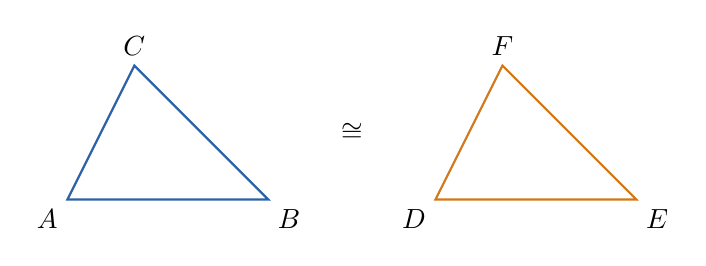
\begin{tikzpicture}[scale=0.85]
  % 三角形ABC
  \coordinate (A) at (0,0);
  \coordinate (B) at (3,0);
  \coordinate (C) at (1,2);
  \draw[thick, mainblue] (A)--(B)--(C)--cycle;
  \node[below left] at (A) {$A$};
  \node[below right] at (B) {$B$};
  \node[above] at (C) {$C$};

  % 三角形DEF
  \coordinate (D) at (5.5,0);
  \coordinate (E) at (8.5,0);
  \coordinate (F) at (6.5,2);
  \draw[thick, examorange] (D)--(E)--(F)--cycle;
  \node[below left] at (D) {$D$};
  \node[below right] at (E) {$E$};
  \node[above] at (F) {$F$};

  \node at (4.25,1) {$\cong$};
\end{tikzpicture}
\end{center}
\end{knowledgebox}

\begin{knowledgebox}[全等三角形的性质]
\begin{enumerate}[nosep]
  \item 全等三角形的\textbf{对应边相等}。
  \item 全等三角形的\textbf{对应角相等}。
\end{enumerate}

若 $\triangle ABC \cong \triangle DEF$，则：
\[
AB = DE, \quad BC = EF, \quad AC = DF
\]
\[
\angle A = \angle D, \quad \angle B = \angle E, \quad \angle C = \angle F
\]

\textbf{注意：}写全等时，对应顶点必须写在对应位置。$\triangle ABC \cong \triangle DEF$ 表示 $A \leftrightarrow D$，$B \leftrightarrow E$，$C \leftrightarrow F$。
\end{knowledgebox}

\begin{warnbox}[易错提醒]
\textbf{书写全等三角形时，对应顶点必须写在对应位置！}

如果 $\triangle ABC \cong \triangle DEF$，则 $AB$ 对应 $DE$，而不是 $AB$ 对应 $EF$。写错对应关系会导致后续推理全部出错。

判断对应关系的方法：
\begin{itemize}[nosep]
  \item 对应角相等 $\rightarrow$ 确定对应顶点。
  \item 对应边相等 $\rightarrow$ 确定对应顶点。
  \item 公共边、公共角往往是对应元素。
\end{itemize}
\end{warnbox}

% ---- 12.2 全等三角形的判定 ----
\subsection*{12.2\quad 全等三角形的判定}

\begin{knowledgebox}[全等三角形的判定方法]
\begin{enumerate}[nosep]
  \item \textbf{SSS（边边边）：}三边分别相等的两个三角形全等。
  \item \textbf{SAS（边角边）：}两边和它们的夹角分别相等的两个三角形全等。
  \item \textbf{ASA（角边角）：}两角和它们的夹边分别相等的两个三角形全等。
  \item \textbf{AAS（角角边）：}两角和其中一个角的对边分别相等的两个三角形全等。
  \item \textbf{HL（斜边直角边）：}斜边和一条直角边分别相等的两个直角三角形全等。
\end{enumerate}
\end{knowledgebox}

\begin{center}
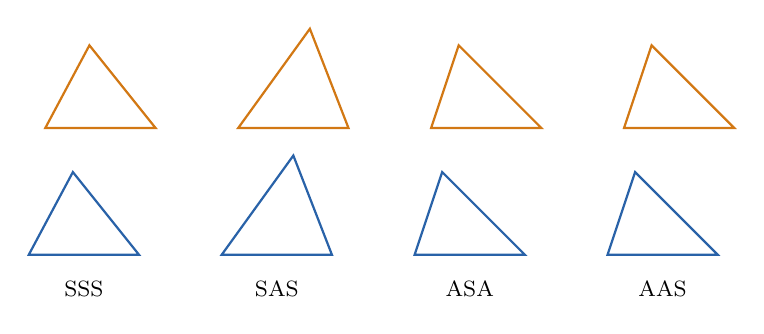
\begin{tikzpicture}[scale=0.7]
  % SSS
  \draw[thick, mainblue] (0,0)--(2,0)--(0.8,1.5)--cycle;
  \node[below] at (1,-0.3) {\footnotesize SSS};
  \draw[thick, examorange] (0.3,2.3)--(2.3,2.3)--(1.1,3.8)--cycle;

  % SAS
  \draw[thick, mainblue] (3.5,0)--(5.5,0)--(4.8,1.8)--cycle;
  \node[below] at (4.5,-0.3) {\footnotesize SAS};
  \draw[thick, examorange] (3.8,2.3)--(5.8,2.3)--(5.1,4.1)--cycle;

  % ASA
  \draw[thick, mainblue] (7,0)--(9,0)--(7.5,1.5)--cycle;
  \node[below] at (8,-0.3) {\footnotesize ASA};
  \draw[thick, examorange] (7.3,2.3)--(9.3,2.3)--(7.8,3.8)--cycle;

  % AAS
  \draw[thick, mainblue] (10.5,0)--(12.5,0)--(11,1.5)--cycle;
  \node[below] at (11.5,-0.3) {\footnotesize AAS};
  \draw[thick, examorange] (10.8,2.3)--(12.8,2.3)--(11.3,3.8)--cycle;
\end{tikzpicture}
\end{center}

\begin{warnbox}[重要提醒]
\textbf{SSA（边边角）不能判定全等！}两边和其中一边的对角分别相等的两个三角形不一定全等。如下图，$\triangle ABC$ 和 $\triangle ABD$ 满足 $AB = AB$，$AC = AD$，$\angle B = \angle B$，但它们不全等。

\begin{center}
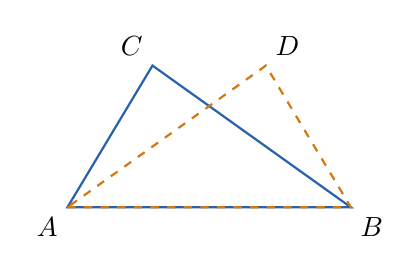
\begin{tikzpicture}[scale=0.9]
  \coordinate (A) at (0,0);
  \coordinate (B) at (4,0);
  \coordinate (C) at (1.2,2);
  \coordinate (D) at (2.8,2);
  \draw[thick, mainblue] (A)--(B)--(C)--cycle;
  \draw[thick, examorange, dashed] (A)--(B)--(D)--cycle;
  \node[below left] at (A) {$A$};
  \node[below right] at (B) {$B$};
  \node[above left] at (C) {$C$};
  \node[above right] at (D) {$D$};
\end{tikzpicture}
\end{center}
\end{warnbox}

\begin{warnbox}[易错提醒]
\textbf{SAS 中的"A"必须是两边的夹角！}如果角不是夹角，就变成了 SSA，不能判定全等。

\textbf{ASA 中的"S"必须是两角的夹边！}如果边不是夹边，就变成了 AAA，不能判定全等（AAA 只能说明形状相同，大小可能不同）。
\end{warnbox}

\begin{tipbox}[判定方法选择口诀]
\begin{itemize}[nosep]
  \item 已知三边 $\rightarrow$ SSS
  \item 已知两边 $\rightarrow$ 找夹角（SAS），不能用对角（SSA 不行）
  \item 已知两角 $\rightarrow$ 找夹边（ASA）或对边（AAS）
  \item 直角三角形 $\rightarrow$ 还可用 HL
  \item 只有三个角 $\rightarrow$ AAA 不行！
\end{itemize}
\end{tipbox}

% ---- 12.3 角平分线的性质 ----
\subsection*{12.3\quad 角平分线的性质}

\begin{knowledgebox}[角平分线的性质定理]
\textbf{定理：}角的平分线上的点到角的两边的距离相等。

\begin{center}
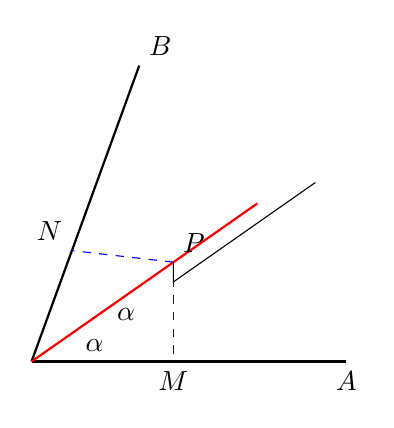
\begin{tikzpicture}[scale=1.0]
  \coordinate (O) at (0,0);
  \coordinate (A) at (4,0);
  \coordinate (B) at ({4*cos(70)},{4*sin(70)});
  \coordinate (P) at ({2.2*cos(35)},{2.2*sin(35)});
  \coordinate (M) at ({2.2*cos(35)},0);
  \coordinate (N) at ({1.5*cos(70)},{1.5*sin(70)}); % projection of P onto OB simplified

  \draw[thick] (O)--(A);
  \draw[thick] (O)--(B);
  \draw[thick, red] (O)--({3.5*cos(35)},{3.5*sin(35)});
  \draw[blue, dashed] (P)--(M);
  \draw[blue, dashed] (P)--(N);

  \node[below] at (A) {$A$};
  \node[above right] at (B) {$B$};
  \node[above right] at (P) {$P$};
  \node[below] at (M) {$M$};
  \node[above left] at (N) {$N$};

  \node at (0.8,0.2) {$\alpha$};
  \node at (1.2,0.6) {$\alpha$};

  \draw (P)--++(0,-0.25)--++(M |- P) coordinate (temp); % right angle mark simplified
\end{tikzpicture}
\end{center}

若 $OC$ 是 $\angle AOB$ 的平分线，$P$ 在 $OC$ 上，$PM \perp OA$ 于 $M$，$PN \perp OB$ 于 $N$，则：
\[
PM = PN
\]
\end{knowledgebox}

\begin{knowledgebox}[角平分线的判定定理]
\textbf{逆定理：}角的内部到角的两边距离相等的点在角的平分线上。

若 $PM \perp OA$，$PN \perp OB$，且 $PM = PN$，则 $P$ 在 $\angle AOB$ 的平分线上。
\end{knowledgebox}

\begin{tipbox}[性质与判定的区别]
\begin{itemize}[nosep]
  \item \textbf{性质：}已知点在角平分线上 $\rightarrow$ 推出距离相等。
  \item \textbf{判定：}已知距离相等 $\rightarrow$ 推出点在角平分线上。
\end{itemize}
性质和判定互为逆命题，注意区分使用场景。
\end{tipbox}

% ---- 12.4 证明全等的书写格式 ----
\subsection*{12.4\quad 证明全等的书写格式}

\begin{knowledgebox}[标准书写格式]
证明两个三角形全等时，应按照以下格式书写：

\textbf{第一步：}明确指出要证明哪两个三角形全等。

\textbf{第二步：}列出证明全等所需的三个条件（对应边或对应角相等），每个条件都要写明理由。

\textbf{第三步：}用判定方法写出结论。

\textbf{示例格式：}
\begin{quote}
在 $\triangle ABC$ 和 $\triangle DEF$ 中，

$\because\ AB = DE$（已知）\\
$\quad\ \angle B = \angle E$（已知）\\
$\quad\ BC = EF$（已知）

$\therefore\ \triangle ABC \cong \triangle DEF$（SAS）
\end{quote}
\end{knowledgebox}

\begin{warnbox}[书写规范提醒]
\begin{itemize}[nosep]
  \item 对应顶点写在对应位置：$\triangle ABC \cong \triangle DEF$，不能写成 $\triangle ABC \cong \triangle EFD$。
  \item 每个等式后面都要注明理由（已知、公共边、对顶角、中点定义等）。
  \item 最后用判定定理（SSS/SAS/ASA/AAS/HL）写出结论。
\end{itemize}
\end{warnbox}

% ============================================================
%  第二部分：例题精讲
% ============================================================
\section*{\textcolor{examorange}{二、例题精讲}}

\begin{examplebox}[【例题1】基础计算——利用全等求边长和角度]
如图，$\triangle ABC \cong \triangle ADE$，$\angle B = 40°$，$\angle E = 60°$，$AB = 5$，$BC = 7$。求 $\angle A$ 的度数以及 $AD$ 和 $DE$ 的长度。

\begin{center}
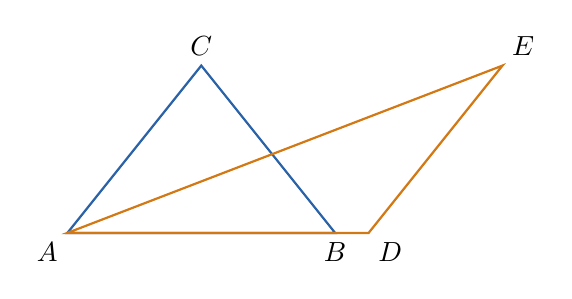
\begin{tikzpicture}[scale=0.85]
  \coordinate (A) at (0,0);
  \coordinate (B) at (4,0);
  \coordinate (C) at (2,2.5);
  \coordinate (D) at (4.5,0);
  \coordinate (E) at (6.5,2.5);
  \draw[thick, mainblue] (A)--(B)--(C)--cycle;
  \draw[thick, examorange] (A)--(D)--(E)--cycle;
  \node[below left] at (A) {$A$};
  \node[below] at (B) {$B$};
  \node[above] at (C) {$C$};
  \node[below right] at (D) {$D$};
  \node[above right] at (E) {$E$};
\end{tikzpicture}
\end{center}
\end{examplebox}

\textbf{解：}

$\because\ \triangle ABC \cong \triangle ADE$

$\therefore$ 对应关系为 $A \leftrightarrow A$，$B \leftrightarrow D$，$C \leftrightarrow E$。

由全等三角形性质：
\[
AD = AB = 5, \quad DE = BC = 7, \quad \angle D = \angle B = 40°, \quad \angle E = \angle C = 60°
\]

在 $\triangle ABC$ 中：
\[
\angle A = 180° - \angle B - \angle C = 180° - 40° - 60° = 80°
\]

所以 $\angle A = 80°$，$AD = 5$，$DE = 7$。

\begin{tipbox}[方法总结]
利用全等求边长和角度，关键是找准对应关系。根据已知的全等记号 $\triangle ABC \cong \triangle ADE$，按字母顺序一一对应即可。
\end{tipbox}

\begin{examplebox}[【例题2】基础证明——SSS 判定全等]
如图，$AB = CD$，$AC = BD$。求证：$\triangle ABC \cong \triangle DCB$。

\begin{center}
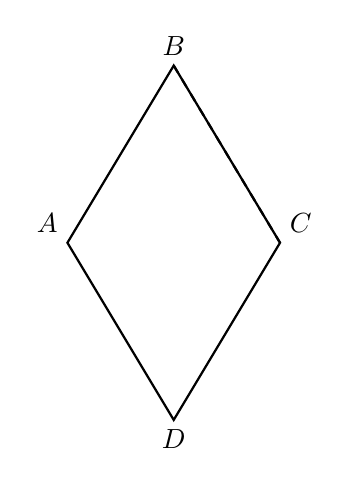
\begin{tikzpicture}[scale=0.9]
  \coordinate (A) at (-1.5,0);
  \coordinate (B) at (0,2.5);
  \coordinate (C) at (1.5,0);
  \coordinate (D) at (0,-2.5);
  \draw[thick] (A)--(B)--(C)--(D)--cycle;
  \draw[thick, dashed] (B)--(C);
  \node[above left] at (A) {$A$};
  \node[above] at (B) {$B$};
  \node[above right] at (C) {$C$};
  \node[below] at (D) {$D$};
\end{tikzpicture}
\end{center}
\end{examplebox}

\textbf{证明：}

\textbf{已知：}$AB = CD$，$AC = BD$。

\textbf{求证：}$\triangle ABC \cong \triangle DCB$。

\textbf{证明：}

在 $\triangle ABC$ 和 $\triangle DCB$ 中，

$\because\ AB = DC$（已知）\\
$\quad\ AC = DB$（已知）\\
$\quad\ BC = CB$（公共边）

$\therefore\ \triangle ABC \cong \triangle DCB$（SSS）

\begin{tipbox}[方法总结]
SSS 判定中，\textbf{公共边}是常用的隐含条件。两个三角形共用的那条边，本身就是相等的。找公共边、公共角、对顶角是证明全等的基本功。
\end{tipbox}

\begin{examplebox}[【例题3】证明题——SAS 判定全等]
如图，已知 $AB = AC$，$AD = AE$，$\angle BAD = \angle CAE$。求证：$\triangle ABD \cong \triangle ACE$。

\begin{center}
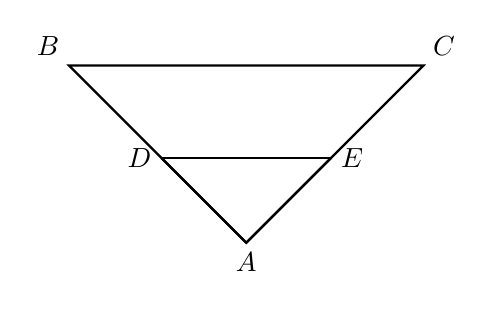
\begin{tikzpicture}[scale=0.9]
  \coordinate (A) at (0,0);
  \coordinate (B) at (-2.5,2.5);
  \coordinate (C) at (2.5,2.5);
  \coordinate (D) at (-1.2,1.2);
  \coordinate (E) at (1.2,1.2);
  \draw[thick] (A)--(B)--(C)--cycle;
  \draw[thick] (A)--(D);
  \draw[thick] (A)--(E);
  \draw[thick] (D)--(E);
  \node[below] at (A) {$A$};
  \node[above left] at (B) {$B$};
  \node[above right] at (C) {$C$};
  \node[left] at (D) {$D$};
  \node[right] at (E) {$E$};
\end{tikzpicture}
\end{center}
\end{examplebox}

\textbf{证明：}

\textbf{已知：}$AB = AC$，$AD = AE$，$\angle BAD = \angle CAE$。

\textbf{求证：}$\triangle ABD \cong \triangle ACE$。

\textbf{证明：}

$\because\ \angle BAD = \angle CAE$（已知）

$\therefore\ \angle BAD + \angle DAC = \angle CAE + \angle DAC$（等式性质）

即 $\angle BAC = \angle DAE$ \quad（此处注意：$\angle BAC = \angle BAD + \angle DAC$）

在 $\triangle ABD$ 和 $\triangle ACE$ 中，

$\because\ AB = AC$（已知）\\
$\quad\ \angle BAD = \angle CAE$（已知）\\
$\quad\ AD = AE$（已知）

$\therefore\ \triangle ABD \cong \triangle ACE$（SAS）

\begin{tipbox}[方法总结]
SAS 判定要求角必须是\textbf{两边的夹角}。本题中，$\angle BAD$ 是 $AB$ 和 $AD$ 的夹角，$\angle CAE$ 是 $AC$ 和 $AE$ 的夹角，正好满足 SAS 条件。如果角不是夹角，就不能用 SAS。
\end{tipbox}

\begin{examplebox}[【例题4】证明题——ASA 与 AAS 判定全等]
如图，$AB \parallel CD$，$AB = CD$，点 $E$、$F$ 在线段 $AC$ 上，且 $AE = CF$。求证：$\triangle ABE \cong \triangle CDF$。

\begin{center}
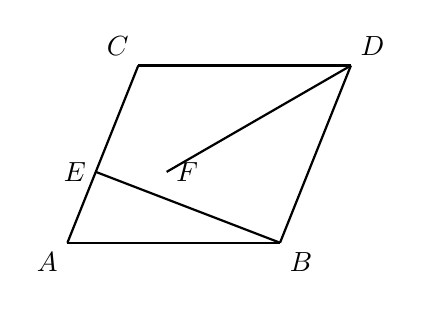
\begin{tikzpicture}[scale=0.9]
  \coordinate (A) at (0,0);
  \coordinate (B) at (3,0);
  \coordinate (C) at (1,2.5);
  \coordinate (D) at (4,2.5);
  \coordinate (E) at (0.4,1);
  \coordinate (F) at (1.4,1);
  \draw[thick] (A)--(B);
  \draw[thick] (C)--(D);
  \draw[thick] (A)--(C);
  \draw[thick] (B)--(D);
  \draw[thick] (B)--(E);
  \draw[thick] (D)--(F);
  \node[below left] at (A) {$A$};
  \node[below right] at (B) {$B$};
  \node[above left] at (C) {$C$};
  \node[above right] at (D) {$D$};
  \node[left] at (E) {$E$};
  \node[right] at (F) {$F$};
\end{tikzpicture}
\end{center}
\end{examplebox}

\textbf{证明：}

\textbf{已知：}$AB \parallel CD$，$AB = CD$，$AE = CF$。

\textbf{求证：}$\triangle ABE \cong \triangle CDF$。

\textbf{证明：}

$\because\ AB \parallel CD$（已知）

$\therefore\ \angle BAC = \angle DCA$（两直线平行，内错角相等）

在 $\triangle ABE$ 和 $\triangle CDF$ 中，

$\because\ \angle BAE = \angle DCF$（已证）\\
$\quad\ AB = CD$（已知）\\
$\quad\ \angle ABE = \angle CDF$（两直线平行，内错角相等）

$\therefore\ \triangle ABE \cong \triangle CDF$（ASA）

\textbf{另解（AAS）：}也可以用 $\angle BAE = \angle DCF$，$AB = CD$，$\angle AEB = \angle CFD$（对顶角相等），由 AAS 判定。

\begin{tipbox}[方法总结]
遇到平行线，立刻想到内错角相等、同位角相等、同旁内角互补。这些角度关系是证明全等时获取角相等条件的重要来源。
\end{tipbox}

\begin{examplebox}[【例题5】综合提高——利用全等证明线段相等]
如图，$AD$ 是 $\triangle ABC$ 的中线，$E$ 是 $AD$ 延长线上一点，且 $DE = AD$。连接 $BE$。求证：$BE = AC$，$BE \parallel AC$。

\begin{center}
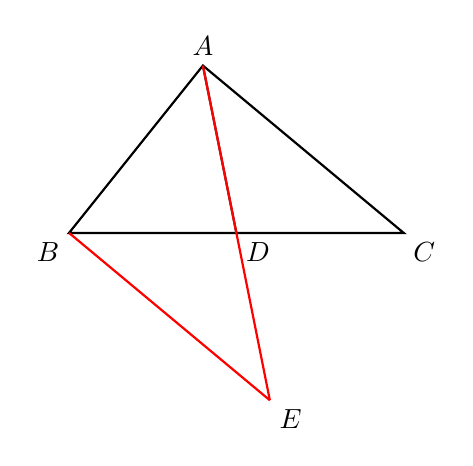
\begin{tikzpicture}[scale=0.85]
  \coordinate (A) at (0,2.5);
  \coordinate (B) at (-2,0);
  \coordinate (C) at (3,0);
  \coordinate (D) at (0.5,0);
  \coordinate (E) at (1,-2.5);
  \draw[thick] (A)--(B)--(C)--cycle;
  \draw[thick] (A)--(D);
  \draw[thick, red] (A)--(E);
  \draw[thick, red] (B)--(E);
  \node[above] at (A) {$A$};
  \node[below left] at (B) {$B$};
  \node[below right] at (C) {$C$};
  \node[below right] at (D) {$D$};
  \node[below right] at (E) {$E$};
\end{tikzpicture}
\end{center}
\end{examplebox}

\textbf{证明：}

\textbf{已知：}$D$ 是 $BC$ 的中点（即 $BD = DC$），$DE = AD$。

\textbf{求证：}$BE = AC$，$BE \parallel AC$。

\textbf{证明：}

在 $\triangle BDE$ 和 $\triangle CDA$ 中，

$\because\ BD = CD$（$D$ 是 $BC$ 的中点）\\
$\quad\ \angle BDE = \angle CDA$（对顶角相等）\\
$\quad\ DE = DA$（已知）

$\therefore\ \triangle BDE \cong \triangle CDA$（SAS）

$\therefore\ BE = AC$（全等三角形对应边相等）

$\therefore\ \angle BED = \angle CAD$（全等三角形对应角相等）

$\therefore\ BE \parallel AC$（内错角相等，两直线平行）

\begin{tipbox}[方法总结]
利用全等证明线段相等或平行，关键步骤是：(1) 找到包含目标线段的两个三角形；(2) 证明这两个三角形全等；(3) 由全等的性质推出结论。遇到中点条件，往往能提供等边关系。
\end{tipbox}

\begin{examplebox}[【例题6】易错辨析——为什么 SSA 不能判定全等]
小华说："已知两边和其中一边的对角相等，两个三角形一定全等。"请举反例说明小华的说法是错误的。
\end{examplebox}

\textbf{解：}

构造反例如下：

设 $\angle B = 30°$，$AB = 4$，$AC = 2$。

以 $A$ 为圆心、$AC = 2$ 为半径画弧，与射线 $BC$ 可能有两个交点 $C_1$ 和 $C_2$：

\begin{center}
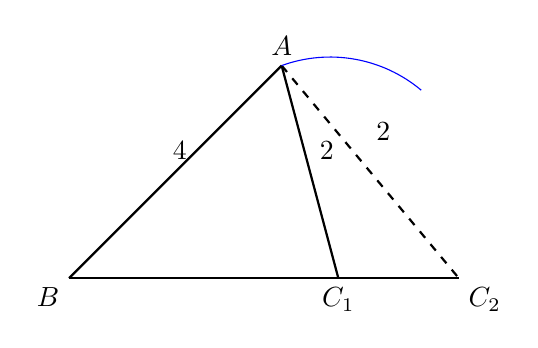
\begin{tikzpicture}[scale=0.9]
  \coordinate (A) at (0,3);
  \coordinate (B) at (-3,0);
  \coordinate (C1) at (0.8,0);
  \coordinate (C2) at (2.5,0);
  \draw[thick] (A)--(B);
  \draw[thick] (A)--(C1);
  \draw[thick, dashed] (A)--(C2);
  \draw[thick] (B)--(C2);
  \node[above] at (A) {$A$};
  \node[below left] at (B) {$B$};
  \node[below] at (C1) {$C_1$};
  \node[below right] at (C2) {$C_2$};
  \node[left] at (-1.2,1.8) {$4$};
  \node[right] at (0.4,1.8) {$2$};
  \node[above right] at (1.2,1.8) {$2$};
  \draw[blue] (A) arc[start angle=110, end angle=50, radius=2];
\end{tikzpicture}
\end{center}

$\triangle ABC_1$ 和 $\triangle ABC_2$ 满足：
\begin{itemize}[nosep]
  \item $AB = AB$（公共边）
  \item $AC_1 = AC_2 = 2$
  \item $\angle B = \angle B = 30°$
\end{itemize}

即两边和其中一边的对角分别相等，但 $\triangle ABC_1 \not\cong \triangle ABC_2$（$BC_1 \neq BC_2$）。

所以小华的说法是错误的，SSA 不能判定全等。

\begin{warnbox}[易错提醒]
SSA 不是判定方法！特别要注意 SAS 中的角必须是\textbf{夹角}（两边中间的那个角），而不是对角。
\end{warnbox}

\begin{examplebox}[【例题7】综合提高——角平分线性质的运用]
如图，在 $\triangle ABC$ 中，$\angle C = 90°$，$AD$ 平分 $\angle BAC$，$DE \perp AB$ 于 $E$，$BC = 8$，$BD = 5$。求 $DE$ 的长度。

\begin{center}
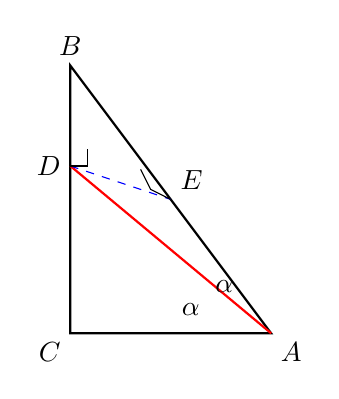
\begin{tikzpicture}[scale=0.85]
  \coordinate (C) at (0,0);
  \coordinate (B) at (0,4);
  \coordinate (A) at (3,0);
  \coordinate (D) at (0,2.5);
  \coordinate (E) at (1.5,2);
  \draw[thick] (C)--(B)--(A)--cycle;
  \draw[thick, red] (A)--(D);
  \draw[blue, dashed] (D)--(E);
  \node[below left] at (C) {$C$};
  \node[above] at (B) {$B$};
  \node[below right] at (A) {$A$};
  \node[left] at (D) {$D$};
  \node[above right] at (E) {$E$};
  \draw (D)--++(0.25,0)--++(0,0.25);
  \draw (E)--++(-0.3,0.15)--++(-0.15,0.3);
  \node at (1.8,0.35) {$\alpha$};
  \node at (2.3,0.7) {$\alpha$};
\end{tikzpicture}
\end{center}
\end{examplebox}

\textbf{解：}

$\because\ AD$ 平分 $\angle BAC$，$\angle C = 90°$，$DE \perp AB$

$\therefore$ 点 $D$ 在角平分线 $AD$ 上，$DC \perp AC$（$\angle C = 90°$），$DE \perp AB$

由角平分线的性质：角平分线上的点到角两边的距离相等。

$\therefore\ DE = DC$

又 $\because\ DC = BC - BD = 8 - 5 = 3$

$\therefore\ DE = 3$

\begin{tipbox}[方法总结]
利用角平分线性质求距离，核心思路是：角平分线上的点到角两边的\textbf{垂直距离}相等。注意必须是垂直距离，不是任意距离。本题中 $DC \perp AC$（因为 $\angle C = 90°$），$DE \perp AB$，所以 $DE = DC$。
\end{tipbox}

\begin{examplebox}[【例题8】与第11章交叉的综合题]
如图，在 $\triangle ABC$ 中，$\angle B = 2\angle C$，$AD$ 是 $\angle BAC$ 的平分线，$AD = AB$。求 $\angle C$ 的度数。

\begin{center}
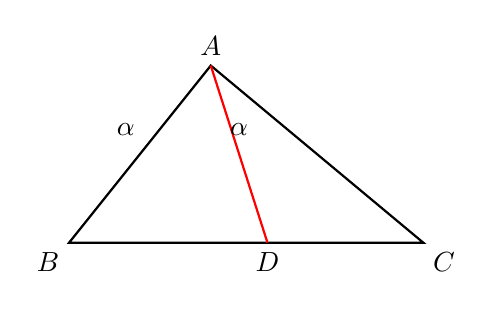
\begin{tikzpicture}[scale=0.9]
  \coordinate (A) at (0,2.5);
  \coordinate (B) at (-2,0);
  \coordinate (C) at (3,0);
  \coordinate (D) at (0.8,0);
  \draw[thick] (A)--(B)--(C)--cycle;
  \draw[thick, red] (A)--(D);
  \node[above] at (A) {$A$};
  \node[below left] at (B) {$B$};
  \node[below right] at (C) {$C$};
  \node[below] at (D) {$D$};
  \node at (-1.2,1.6) {$\alpha$};
  \node at (0.4,1.6) {$\alpha$};
\end{tikzpicture}
\end{center}
\end{examplebox}

\textbf{解：}

设 $\angle C = x$，则 $\angle B = 2x$。

由三角形内角和：$\angle BAC = 180° - \angle B - \angle C = 180° - 2x - x = 180° - 3x$。

$\because\ AD$ 平分 $\angle BAC$

$\therefore\ \angle BAD = \angle DAC = \dfrac{180° - 3x}{2}$

$\because\ AB = AD$（已知）

$\therefore\ \triangle ABD$ 是等腰三角形，$\angle ADB = \angle ABD = \angle B = 2x$

在 $\triangle ABD$ 中，由内角和：
\[
\angle BAD + \angle ABD + \angle ADB = 180°
\]
\[
\frac{180° - 3x}{2} + 2x + 2x = 180°
\]
\[
\frac{180° - 3x}{2} + 4x = 180°
\]
\[
180° - 3x + 8x = 360°
\]
\[
5x = 180°
\]
\[
x = 36°
\]

所以 $\angle C = 36°$。

\textbf{验证：}$\angle C = 36°$，$\angle B = 72°$，$\angle BAC = 180° - 72° - 36° = 72°$，$\angle BAD = 36°$，$\angle ADB = 72°$。在 $\triangle ABD$ 中，$36° + 72° + 72° = 180°$，$\triangle ABD$ 确实是等腰三角形，$AB = AD$。验证正确。

\begin{tipbox}[方法总结]
本题综合运用了第11章的内角和定理、等腰三角形性质以及角平分线定义。解综合题的关键是设未知数，利用多个定理建立方程求解。
\end{tipbox}

% ============================================================
%  第三部分：应用题
% ============================================================
\section*{\textcolor{apppurple}{三、应用题}}

\begin{appbox}[【应用1】工程测量中的全等三角形]
工程师需要测量一条河的宽度（$AB$），但无法直接跨河测量。他在河岸一侧选择了点 $C$，使得 $AC \perp AB$；在 $AC$ 上取点 $D$，使 $CD = AC$；再在河对岸找一点 $E$，使 $E$、$D$、$B$ 三点共线。已知测量得 $AC = 30\text{ m}$，$DE = 50\text{ m}$，求河宽 $AB$。

\begin{center}
\begin{tikzpicture}[scale=0.7]
  \fill[blue!10] (0,0)--(7,0)--(7,-0.8)--(0,-0.8)--cycle;
  \node at (3.5,-0.4) {\small 河流};
  \coordinate (A) at (0,0);
  \coordinate (B) at (7,0);
  \coordinate (C) at (0,4);
  \coordinate (D) at (0,8);
  \coordinate (E) at (7,0);
  \draw[thick] (A)--(C)--(D);
  \draw[thick] (D)--(B);
  \draw[dashed] (A)--(B);
  \node[below left] at (A) {$A$};
  \node[below right] at (B) {$B$};
  \node[left] at (C) {$C$};
  \node[above left] at (D) {$D$};
  \node[below right] at (E) {$E$};
  \draw (0,0.3)--(0.3,0.3)--(0.3,0);
\end{tikzpicture}
\end{center}
\end{appbox}

\textbf{解：}

$\because\ AC \perp AB$，$\therefore\ \angle A = 90°$

在 $\triangle CAB$ 和 $\triangle CDE$ 中：

$\because\ AC = DC$（已知 $CD = AC = 30\text{ m}$）\\
$\quad\ \angle CAB = \angle CDE$（对顶角相等，$E$、$D$、$B$ 共线且 $\angle A = 90°$）

实际上更直接地：

$\because\ \angle CAB = \angle CDE = 90°$（$AC \perp AB$，且 $E$、$D$、$B$ 共线）

等等，让我重新分析。$D$ 在 $AC$ 的延长线上，$E$、$D$、$B$ 三点共线。

在 $\triangle ACB$ 和 $\triangle DCE$ 中：

$\because\ AC = DC = 30$（已知）\\
$\quad\ \angle ACB = \angle DCE$（对顶角相等）\\
$\quad\ \angle CAB = \angle CDE$（两直线平行则内错角相等……）

简化思路：$\angle A = \angle D = 90°$（若 $AC \perp AB$ 且 $E$、$D$、$B$ 共线），则直角三角形全等的条件：

$\because\ \angle A = \angle D = 90°$，$AC = DC = 30$，$\angle ACB = \angle DCE$（对顶角）

$\therefore\ \triangle ACB \cong \triangle DCE$（ASA）

$\therefore\ AB = DE = 50\text{ m}$

所以河宽 $AB = 50\text{ m}$。

\begin{appbox}[【应用2】利用全等验证零件质量]
质检员要检验一个三角形零件 $\triangle PQR$ 是否合格。标准要求 $PQ = 10\text{ cm}$，$PR = 8\text{ cm}$，$\angle P = 60°$。质检员用卡尺量得 $PQ = 10\text{ cm}$，$PR = 8\text{ cm}$，并用量角器测得 $\angle P = 60°$。请问质检员能否判定该零件合格？请说明理由。
\end{appbox}

\textbf{解：}

质检员可以判定该零件合格。

\textbf{理由：}根据 SAS 判定定理，两边和它们的夹角分别相等的两个三角形全等。

已知零件满足：$PQ = 10\text{ cm}$，$PR = 8\text{ cm}$，$\angle P = 60°$，与标准要求完全一致。

根据 SAS，该零件 $\triangle PQR$ 与标准三角形全等，因此形状和大小完全一致，零件合格。

实际应用中，如果零件形状复杂，可以用三坐标测量机测量关键点的坐标，再通过 SSS 或 SAS 来验证是否与设计图纸一致。

\begin{appbox}[【应用3】利用角平分线性质解决道路设计问题]
如图，两条公路 $OA$ 和 $OB$ 交于点 $O$，形成一个角。现要在角的内部（公路围成的区域内）建一个加油站 $P$，要求加油站到两条公路的距离相等，且距两条公路的距离不超过 $200\text{ m}$。请问加油站应建在什么位置？如果额外要求加油站距离路口 $O$ 为 $150\text{ m}$，这样的加油站位置是否唯一？

\begin{center}
\begin{tikzpicture}[scale=0.8]
  \coordinate (O) at (0,0);
  \coordinate (A) at (5,0);
  \coordinate (B) at ({3*cos(55)},{3*sin(55)});
  \draw[thick] (O)--(A);
  \draw[thick] (O)--(B);
  \node[below] at (A) {$A$（公路）};
  \node[above right] at (B) {$B$（公路）};
  \node[below left] at (O) {$O$};
  \draw[red, dashed] (O)--({3*cos(27.5)},{3*sin(27.5)});
  \node[red, above right] at ({1.5*cos(27.5)},{1.5*sin(27.5)}) {角平分线};
\end{tikzpicture}
\end{center}
\end{appbox}

\textbf{解：}

\textbf{第一问：}

由角平分线的性质：角平分线上的点到角两边的距离相等。

所以加油站 $P$ 应建在 $\angle AOB$ 的角平分线上（角的内部区域）。

又要求距离不超过 $200\text{ m}$，所以 $P$ 在角平分线上、距 $O$ 不超过 $200\text{ m}$ 的范围内。

\textbf{第二问：}

如果要求加油站距路口 $O$ 为 $150\text{ m}$，则 $P$ 在角平分线上距 $O$ 恰好 $150\text{ m}$ 处。

在角的内部，角平分线上距 $O$ 为 $150\text{ m}$ 的点只有\textbf{一个}，所以加油站的位置是\textbf{唯一}的。

\begin{tipbox}[方法总结]
角平分线性质的实际应用：到角两边距离相等的点一定在角平分线上。结合距离条件，可以确定具体位置。
\end{tipbox}

% ============================================================
%  第四部分：课堂练习
% ============================================================
\section*{\textcolor{tipgreen}{四、课堂练习}}

\begin{enumerate}
  \item 如图，$AB = AC$，$BD = CE$。求证：$\triangle ABD \cong \triangle ACE$。

\begin{center}
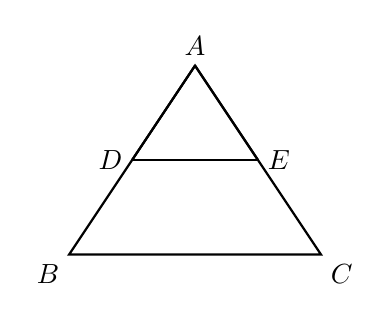
\begin{tikzpicture}[scale=0.8]
  \coordinate (A) at (0,3);
  \coordinate (B) at (-2,0);
  \coordinate (C) at (2,0);
  \coordinate (D) at (-1,1.5);
  \coordinate (E) at (1,1.5);
  \draw[thick] (A)--(B)--(C)--cycle;
  \draw[thick] (A)--(D);
  \draw[thick] (A)--(E);
  \draw[thick] (D)--(E);
  \node[above] at (A) {$A$};
  \node[below left] at (B) {$B$};
  \node[below right] at (C) {$C$};
  \node[left] at (D) {$D$};
  \node[right] at (E) {$E$};
\end{tikzpicture}
\end{center}

  \item 如图，$AB \parallel CD$，$AB = CD$，$E$、$F$ 分别是 $AD$、$BC$ 的中点。求证：$EF \parallel AB$。

\begin{center}
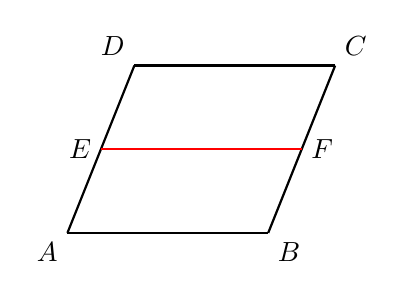
\begin{tikzpicture}[scale=0.85]
  \coordinate (A) at (0,0);
  \coordinate (B) at (3,0);
  \coordinate (D) at (1,2.5);
  \coordinate (C) at (4,2.5);
  \coordinate (E) at (0.5,1.25);
  \coordinate (F) at (3.5,1.25);
  \draw[thick] (A)--(B);
  \draw[thick] (C)--(D);
  \draw[thick] (A)--(D);
  \draw[thick] (B)--(C);
  \draw[thick, red] (E)--(F);
  \node[below left] at (A) {$A$};
  \node[below right] at (B) {$B$};
  \node[above right] at (C) {$C$};
  \node[above left] at (D) {$D$};
  \node[left] at (E) {$E$};
  \node[right] at (F) {$F$};
\end{tikzpicture}
\end{center}

  \item 在 $\triangle ABC$ 中，$\angle C = 90°$，$AD$ 平分 $\angle BAC$，$DE \perp AB$ 于 $E$，$AC = 6$，$BC = 8$。求 $\triangle BDE$ 的周长。

  \item 已知 $\triangle ABC \cong \triangle DEF$，$\triangle ABC$ 的周长为 $24\text{ cm}$，$AB = 7\text{ cm}$，$BC = 8\text{ cm}$。求 $DE$、$EF$、$DF$ 的长度。

  \item 如图，$AC = BD$，$\angle A = \angle D = 90°$。求证：$\triangle ABC \cong \triangle DCB$。

\begin{center}
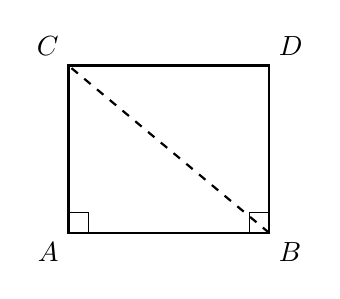
\begin{tikzpicture}[scale=0.85]
  \coordinate (A) at (0,0);
  \coordinate (B) at (3,0);
  \coordinate (C) at (0,2.5);
  \coordinate (D) at (3,2.5);
  \draw[thick] (A)--(B)--(D)--(C)--cycle;
  \draw[thick, dashed] (B)--(C);
  \draw (0,0.3)--(0.3,0.3)--(0.3,0);
  \draw (3,0.3)--(2.7,0.3)--(2.7,0);
  \node[below left] at (A) {$A$};
  \node[below right] at (B) {$B$};
  \node[above left] at (C) {$C$};
  \node[above right] at (D) {$D$};
\end{tikzpicture}
\end{center}
\end{enumerate}

% ---- 参考答案 ----
\begin{knowledgebox}[参考答案]
\textbf{1.} 在 $\triangle ABD$ 和 $\triangle ACE$ 中，

$\because\ AB = AC$（已知），$\angle A = \angle A$（公共角），$BD = CE$（已知）

$\therefore\ \triangle ABD \cong \triangle ACE$（SAS）。

\medskip

\textbf{2.} 连接 $AF$ 并延长，取 $FG = AF$，连接 $CG$。

在 $\triangle ABF$ 和 $\triangle GCF$ 中，$AF = GF$，$\angle AFB = \angle GFC$（对顶角），$BF = CF$（$F$ 是中点），$\therefore\ \triangle ABF \cong \triangle GCF$（SAS）。

$\therefore\ AB = GC$，$\angle BAF = \angle G$。又 $AB \parallel CD$，$AB = CD$，$\therefore\ GC = CD$，$GC \parallel CD$，即 $G$、$C$、$D$ 共线且 $GD \parallel AB$。

在 $\triangle AGD$ 中，$E$ 为 $AD$ 中点，$F$ 为 $AG$ 中点，$\therefore\ EF \parallel GD \parallel AB$（三角形中位线定理）。

\medskip

\textbf{3.} 由勾股定理，$AB = \sqrt{AC^2 + BC^2} = \sqrt{36 + 64} = 10$。

$\because\ AD$ 平分 $\angle BAC$，$DC \perp AC$，$DE \perp AB$，$\therefore\ DE = DC$（角平分线性质）。

$\triangle BDE$ 的周长 $= BD + DE + BE = BD + DC + BE = BC + BE$。

又 $BE = AB - AE = AB - AC = 10 - 6 = 4$（由 $\triangle AED \cong \triangle ACD$（HL）得 $AE = AC$）。

$\therefore$ 周长 $= 8 + 4 = 12$。

\medskip

\textbf{4.} $\triangle ABC$ 周长 $= 24$，$AB = 7$，$BC = 8$，$\therefore\ AC = 24 - 7 - 8 = 9$。

$\because\ \triangle ABC \cong \triangle DEF$，$\therefore\ DE = AB = 7$，$EF = BC = 8$，$DF = AC = 9$。

\medskip

\textbf{5.} 在 $\triangle ABC$ 和 $\triangle DCB$ 中，

$\because\ \angle A = \angle D = 90°$（已知），$AC = DB$（已知），$BC = CB$（公共边）

$\therefore\ \triangle ABC \cong \triangle DCB$（HL）。
\end{knowledgebox}

\vfill
\begin{center}
\small\textcolor{gray}{本讲义仅供教学参考，例题可根据学生水平调整难度。}
\end{center}

\end{document}
